\pdfoutput=1
\documentclass[11pt]{article}
\usepackage[T1]{fontenc}
\usepackage[utf8]{inputenc}
\usepackage{mathptmx}
\usepackage[letterpaper,margin=1in,headheight=14pt]{geometry}
\usepackage{microtype}
\usepackage{amsmath,amssymb,amsthm}
\usepackage{booktabs,tabularx,array,makecell,threeparttable}
\usepackage{graphicx}
\usepackage[font=small,labelfont=bf,skip=6pt,justification=justified]{caption}
\usepackage{xcolor}
\definecolor{accent}{HTML}{2F6DB5}
\usepackage[authoryear,round]{natbib}
\usepackage[colorlinks=true,linkcolor=accent,citecolor=accent,urlcolor=accent]{hyperref}
\hypersetup{pdftitle={Can Demonetization Defeat Grey Capital?},pdfauthor={Thanatchon Chongmankhong},
  pdfkeywords={demonetization, high-denomination banknotes, money laundering, agent-based model, Thailand}}
\usepackage{enumitem}
\usepackage{fancyhdr}
\usepackage{titlesec}

\titleformat{\section}{\normalfont\large\bfseries}{\thesection}{1em}{}
\titleformat{\subsection}{\normalfont\normalsize\bfseries}{\thesubsection}{1em}{}
\titlespacing*{\section}{0pt}{16pt}{7pt}
\titlespacing*{\subsection}{0pt}{11pt}{5pt}
\pagestyle{fancy}\fancyhf{}
\fancyhead[L]{\small\itshape Can Demonetization Defeat Grey Capital?}
\fancyhead[R]{\small\scshape A Preprint -- November 7, 2026}
\fancyfoot[C]{\small\thepage}
\renewcommand{\headrulewidth}{0.4pt}
\fancypagestyle{plain}{\fancyhf{}\fancyfoot[C]{\small\thepage}\renewcommand{\headrulewidth}{0pt}}

\newtheorem{proposition}{Proposition}
\newtheorem{lemma}{Lemma}
\theoremstyle{definition}
\newtheorem{assumption}{Assumption}
\newtheorem{hypothesis}{Hypothesis}
\theoremstyle{remark}
\newtheorem*{remark}{Remark}

\newcolumntype{Y}{>{\raggedright\arraybackslash}X}
\setlength{\tabcolsep}{4pt}
\renewcommand{\arraystretch}{1.15}
\setlist{itemsep=2pt,topsep=4pt}
\newcommand{\figw}{\textwidth}
% float placement: let large tables and figures share pages with text; pack float-only pages from the top
\renewcommand{\topfraction}{0.88}\renewcommand{\bottomfraction}{0.6}
\renewcommand{\textfraction}{0.1}\renewcommand{\floatpagefraction}{0.9}
\setcounter{topnumber}{2}\setcounter{bottomnumber}{2}\setcounter{totalnumber}{4}
\setlength{\floatsep}{12pt plus 2pt minus 2pt}\setlength{\textfloatsep}{14pt plus 3pt minus 3pt}
\setlength{\intextsep}{12pt plus 2pt minus 2pt}
\makeatletter\setlength{\@fptop}{0pt}\setlength{\@fpsep}{14pt}\setlength{\@fpbot}{0pt plus 1fil}\makeatother

\begin{document}
\thispagestyle{plain}
\begin{center}
\vspace*{-0.25in}
\rule{\textwidth}{2.5pt}\par\vspace{12pt}
{\LARGE\bfseries Can Demonetization Defeat Grey Capital?\par}\vspace{8pt}
{\large Evidence, a Calibrated Agent-Based Model, and a Research Agenda\\ for Retiring Thailand's 1,000-Baht Note\par}
\vspace{10pt}\rule{\textwidth}{0.8pt}\par\vspace{18pt}
{\large\bfseries Thanatchon Chongmankhong$^{\ast}$\par}\vspace{6pt}
{\normalsize November 7, 2026\par}
\end{center}
{\renewcommand{\thefootnote}{\fnsymbol{footnote}}\footnotetext[1]{Draft for discussion. All statistics are
approximations that must be verified against primary sources, in particular Bank of Thailand banknote statistics; model
parameters are assumptions, and no live data sources were consulted. References were compiled without database access and
their bibliographic details must be checked. The author acknowledges AI assistance (Claude, Anthropic) in drafting, coding
and figure design. Replication code: \texttt{demonet\_sim\_th.py} (seed 7).}}
\vspace{6pt}
\begin{center}{\large\bfseries Abstract}\end{center}
\vspace{-4pt}
\begin{quote}\small
Proposals to withdraw Thailand's 1,000-baht banknote promise to squeeze grey and black capital, vote buying and
corruption. This paper evaluates that promise by combining a structured synthesis of twelve demonetization episodes, a
cross-country measure of denomination size, and \textit{DemonetSim-TH}, an agent-based model in which illicit holders
choose among direct deposit, structuring through money mules, conversion into alternative stores of value, amnesty and
abandonment under capacity-constrained laundering, while honest holders face a liquidity gap governed by replacement
logistics. The model is calibrated to India's 2016 demonetization by approximate Bayesian computation. Four results stand
out. First, at 0.38 percent of GDP per capita the 1,000-baht note is a mid-sized ``large note'', about a quarter of the
EUR~500 at its withdrawal. Second, an India-style shock destroys or seizes a median of 7.7 percent of illicit cash while
generating about one sixth of India's liquidity disruption, roughly 90 percent of which falls on vulnerable and informal
holders. Third, India's 99.3 percent return rate is consistent with illicit shares between 3 and 29 percent and therefore
does not identify the illicit stock. Fourth, a global sensitivity analysis shows that the bite of any design hinges on
laundering capacity relative to the illicit stock, whereas disruption depends almost entirely on replacement logistics;
a gradual phase-out combined with anti-money-laundering (AML) measures achieves a comparable bite (6.1 percent) at negligible
liquidity cost. We formalize these regularities as a \textit{demonetization trilemma} and propose three identification
strategies to test whether the 1,000-baht note is in fact a preferred medium of illicit exchange.
\end{quote}
\begin{quote}\small
\textbf{Keywords} demonetization $\cdot$ high-denomination banknotes $\cdot$ money laundering $\cdot$ shadow economy
$\cdot$ agent-based modeling $\cdot$ approximate Bayesian computation $\cdot$ Thailand\\[3pt]
\textbf{JEL codes} E41 $\cdot$ E42 $\cdot$ E58 $\cdot$ H26 $\cdot$ K42 $\cdot$ O17 $\cdot$ C63
\end{quote}
\vspace{4pt}

\section{Introduction}

Cash remains the medium of choice for transactions that are meant to leave no trace, and large banknotes make it
especially convenient: one million US dollars in USD~100 notes weighs about ten kilograms, the same value in EUR~500
notes about two \citep{sands2016,rogoff2016}. This observation underlies a series of decisions to retire large notes---the
euro area stopped issuing the EUR~500 in 2019, Canada stopped issuing its CAD~1,000 in 2000 and Singapore its SGD~10,000
in 2014---and, most dramatically, India's overnight demonetization of 86 percent of its currency by value in November 2016.

In Thailand, the idea of withdrawing the 1,000-baht note resurfaces periodically as a remedy for ``grey capital'', ``black
capital'', vote buying and corruption. The argument is intuitive; its empirical premise is not established. India's
experience is sobering: 99.3 percent of the demonetized value returned to the banking system \citep{rbi2018}; the cash
crunch lowered the growth of economic activity by at least two percentage points in the quarter of the shock
\citep{chodorowreich2020}; and although electronic payments expanded \citep{crouzet2023}, the ratio of currency to GDP
returned to its earlier level within a few years \citep{lahiri2020}.

This paper asks three questions. What does international experience imply about the effectiveness and costs of
demonetization as an instrument against illicit wealth? Under alternative designs, how would retiring the 1,000-baht note
affect the stock of illicit cash, the economy and its most vulnerable participants, and the operating costs of the
currency system? And if the policy were pursued, how should it be designed, and which empirical questions must be answered
first?

We proceed in three steps. We synthesize twelve episodes into a typology and six stylized facts, and place the 1,000-baht
note on a cross-country scale of denomination size. We then develop a stylized model in which the state cannot identify
illicit holdings, audit capacity is finite and replacement currency is supplied at a bounded rate. The model yields a
conditional impossibility result, the demonetization trilemma: no design simultaneously destroys a large share of illicit
cash (\textit{bite}), spares honest holders (\textit{smoothness}) and prevents the exchange from becoming a laundering
channel (\textit{integrity}) unless audit capacity exceeds laundering throughput and replacement currency is
pre-positioned in secret. Finally, we quantify the trade-offs with DemonetSim-TH, an agent-based model calibrated to India
2016 by approximate Bayesian computation (ABC), and probe it with a global sensitivity analysis.

The results are summarized in the abstract. Three deserve emphasis. First, the bite of a shock design is small even in
the calibrated model (median 7.7 percent), and its distribution is right-skewed: large bites arise only when illicit
holdings are large relative to the capacity of laundering networks. Second, the most widely cited statistic from
India---the 99.3 percent return rate---rules out large-scale extinguishment but is nearly uninformative about the size of
the illicit stock. Third, the levers that govern the bite (laundering capacity, illicit share, structuring costs) are
disjoint from those that govern disruption (replacement logistics), which is why a phase-out combined with AML measures
dominates a shock: it moves the stock through a tighter net without starving the economy of cash.

The paper contributes to three literatures. It adds a formal and quantitative treatment of the \textit{stock} channel
through which demonetization is supposed to work to a debate dominated by arguments about the \textit{flow} benefits of
retiring large notes \citep{rogoff1998,rogoff2016,sands2016} and by ex post evaluations of India's episode
\citep{chodorowreich2020,lahiri2020,crouzet2023}. It contributes to the economics of crime and money laundering
\citep{becker1968,unger2007} by modeling laundering as a capacity-constrained market, which implies that enforcement
intensity matters far less than laundering capacity once the latter is abundant. And it adds to the measurement
literature on the shadow economy \citep{tanzi1983,schneider2000,medina2018} a non-identification result: aggregate return
rates cannot discriminate between small illicit stocks and large but well-laundered ones.

The analysis also draws on several adjacent literatures. Cash in circulation has risen in many economies despite the
spread of digital payments, largely because cash is held as a store of value \citep{bech2018,jobst2017}, and large notes
are disproportionately hoarded or held abroad \citep{rogoff1998}. Europol documents the role of high-denomination notes in
organized crime \citep{europol2015}, while UNODC describes a shift of laundering in East and Southeast Asia toward casinos,
underground banking and stablecoins \citep{unodc2024}. Work on vote buying emphasizes monitoring and reciprocity rather
than denomination \citep{stokes2005,vicente2014}, and work on corruption stresses measurement challenges that also afflict
the evaluation of demonetization \citep{olken2012}.

Section~\ref{sec:background} reviews international evidence and the Thai setting. Section~\ref{sec:framework} develops the
conceptual framework. Section~\ref{sec:model} describes the model and its calibration, and Section~\ref{sec:results}
reports results. Section~\ref{sec:policy} assesses costs, benefits and designs, and Section~\ref{sec:agenda} sets out a
research agenda. Section~\ref{sec:limits} discusses limitations and Section~\ref{sec:conclusion} concludes.

\section{International evidence and the Thai setting}\label{sec:background}

\subsection{A typology of demonetization}
We classify designs along two dimensions: whether the decision is announced in advance, and whether legal-tender status
lapses at a deadline or persists. Table~\ref{tab:typology} distinguishes four designs; the fourth retains the note but
restricts the use of cash.

\begin{table}[!htbp]\centering\footnotesize
\caption{A typology of demonetization designs}\label{tab:typology}
\begin{tabularx}{\textwidth}{@{}p{3.3cm}Yp{5.6cm}@{}}
\toprule
Design & Defining features & Examples\\
\midrule
A. Shock & Unannounced; legal tender lapses at announcement; short exchange window & India 2016; Venezuela 2016;
Soviet Union 1991; Myanmar 1987\\
B. Announced, short window & Usable until a deadline, then exchanged; often combined with a redesign & Nigeria 2022--23;
Malaysia 1998--99\\
C. Gradual phase-out & Issuance stops; legal tender persists for years or notes remain redeemable indefinitely & Euro
area (EUR 500); Canada (CAD 1,000); Singapore (SGD 10,000); India 2023 (INR 2,000)\\
D. Cash restrictions & Notes retained; caps on cash payments and reporting thresholds & France, Italy, Spain; EU-wide cap
of EUR 10,000 from 2027\\
\bottomrule
\end{tabularx}
\end{table}

\subsection{Twelve episodes}
Table~\ref{tab:episodes} summarizes twelve episodes. The evidence is uneven---rigorous evaluations exist essentially only
for India 2016---so the table should be read as a structured synthesis rather than a meta-analysis.

\begin{table}[!htbp]\centering\footnotesize
\caption{Demonetization episodes}\label{tab:episodes}
\begin{threeparttable}
\begin{tabularx}{\textwidth}{@{}p{2.3cm}p{3.2cm}p{1.6cm}YY@{}}
\toprule
Episode & Notes (share of currency) & Design & Stated aims & Main outcomes\\
\midrule
India 2016 & INR 500 and 1,000 (about 86\%) & A & Black money, counterfeits, terror finance; later cashless
payments & 99.3\% returned; growth at least 2 pp lower in the shock quarter; partly persistent digital adoption\\
Venezuela 2016 & VES 100 & A & Hoarding by cross-border mafias & New notes not ready; unrest; deadline repeatedly
extended\\
Soviet Union 1991 & RUB 50 and 100 & A & Speculation, shadow economy & Three-day exchange with caps; collapse of
confidence\\
Myanmar 1987 & 25, 35 and 75 kyat & A & Black market & No compensation; most money voided; contributed to the 1988
uprising\\
North Korea 2009 & Redenomination 100:1 & A & Private market activity & Savings wiped out; unrest; official reportedly
executed\\
Nigeria 2022--23 & NGN 200, 500, 1,000 (redesign) & B & Counterfeits, hoarding, vote buying, cashless policy & Severe
shortages; protests; Supreme Court extended old notes to end-2023\\
Malaysia 1998--99 & MYR 500 and 1,000 & B & Offshore ringgit, laundering & Limited domestic effects (details to
verify)\\
Euro area 2016--19 & EUR 500 (about 28\%) & C & Illicit use & No disruption; effect on crime not established\\
Canada 2000/2021 & CAD 1,000 & C & Laundering, organized crime & Smooth; legal tender removed in 2021; redeemable\\
Singapore 2014 & SGD 10,000 & C & Laundering risk (preventive) & Smooth\\
United States 1969 & USD 500--10,000 & C & Lack of use & Smooth; still legal tender\\
India 2023 & INR 2,000 (about 11\%) & C & Denomination management & About 97--98\% returned within months; no disruption\\
\bottomrule
\end{tabularx}
\begin{tablenotes}\scriptsize
\item \textit{Notes:} Design letters refer to Table~\ref{tab:typology}. Shares and outcomes are approximate and compiled
from memory; they require verification against central-bank and court documents.
\end{tablenotes}
\end{threeparttable}
\end{table}

Six stylized facts emerge.
\begin{enumerate}[label=\textbf{SF\arabic*.},leftmargin=*]
\item \textit{Returns are near-complete.} Almost all demonetized value returns: 99.3 percent in India 2016
\citep{rbi2018} and about 97--98 percent of the INR 2,000 notes withdrawn in 2023. Section~\ref{sec:ident} shows that high
returns are consistent with small illicit stocks and with large but laundered ones.
\item \textit{Logistics govern disruption.} The crises in India (2016), Venezuela (2016) and Nigeria (2023) were driven
by shortfalls of replacement currency.
\item \textit{Incidence is regressive.} Costs fall on cash-dependent and informal participants
\citep{chodorowreich2020}.
\item \textit{Digital substitution is partial.} Electronic payments rise and some adoption persists
\citep{crouzet2023}, but cash demand rebounds \citep{lahiri2020}.
\item \textit{Gradual withdrawals are cheap but target flows, not stocks.} The euro area, Canada and Singapore
reported no disruption, but also made no attempt to extinguish existing illicit holdings \citep{ecb2016}.
\item \textit{Abrupt designs carry legitimacy risks.} Confiscatory or abrupt designs triggered unrest in Myanmar,
the Soviet Union, North Korea and Venezuela. India's Supreme Court upheld the 2016 decision by four to one, the dissent
holding that it required legislation \citep{scindia2023}; Nigeria's Supreme Court extended the validity of old notes.
\end{enumerate}

\subsection{The Thai setting}
Banknotes in circulation are approximately THB 1.7--2.1 trillion, about 10 percent of GDP, of which the 1,000-baht note
accounts for an estimated 65--80 percent by value; our central value of 72 percent implies a stock of about THB 1.37
trillion, or 1.4 billion notes \citep{bot}. The note is both the workhorse of ATM dispensing and a household store of
value. At roughly USD 28--30 it is worth less than a third of a USD~100 note.

\begin{figure}[!htbp]\centering
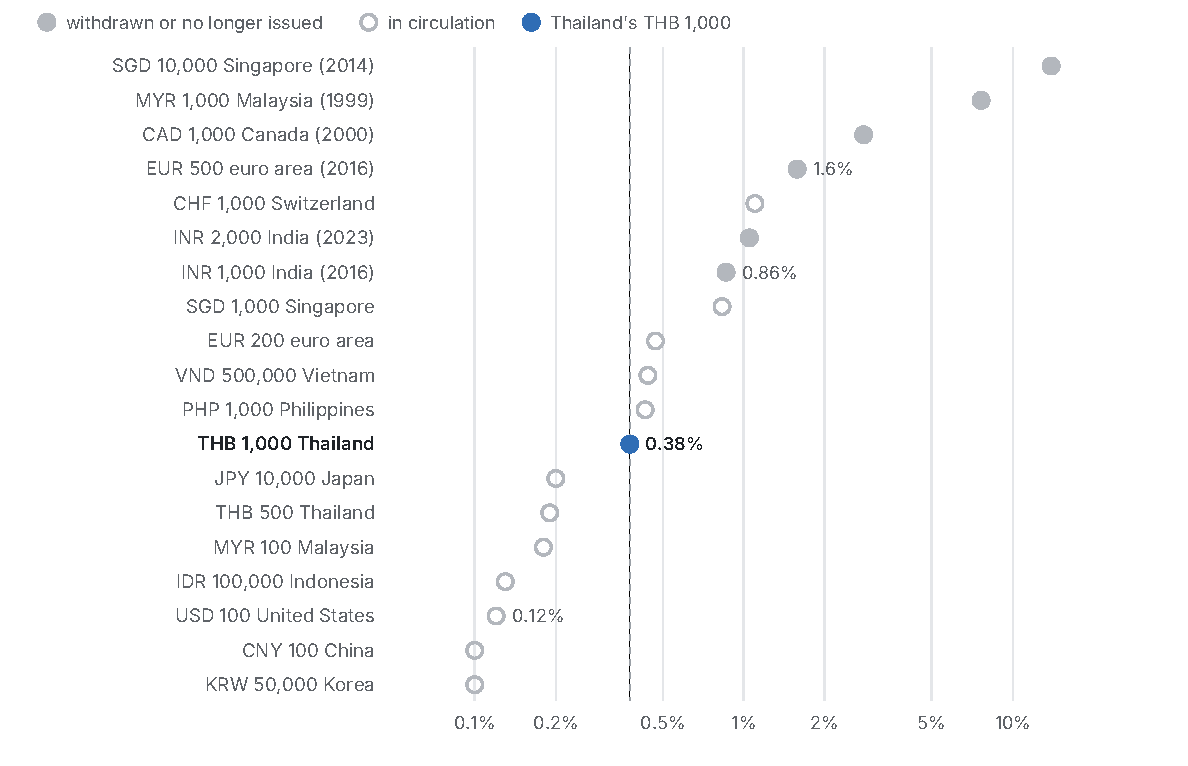
\includegraphics[width=\figw]{figs_en/relvalue.pdf}
\caption{\textbf{The 1,000-baht note is a mid-sized ``large note''.} Face value of one note relative to nominal GDP per capita in the year indicated (log scale). At 0.38\%, the THB~1,000 is about a quarter of the EUR~500 at its withdrawal. Filled grey dots mark notes withdrawn or no longer issued, hollow dots notes in circulation, and the dashed line the THB~1,000. GDP per capita and exchange rates are approximations. Source: \texttt{denomination\_metrics()} in the replication code.}\label{fig:relvalue}
\end{figure}

Figure~\ref{fig:relvalue} places the note on a cross-country scale. At 0.38 percent of GDP per capita---about 1.4 days of
average income---it is comparable to the largest notes of the Philippines and Vietnam but between two and thirty-seven
times smaller, relative to income, than the notes retired in the euro area, Canada, Singapore, Malaysia and India. The
argument that large notes facilitate crime \citep{rogoff2016,sands2016} therefore applies to the 1,000-baht note with much
less force than to the EUR 500. Figure~\ref{fig:bulk} shows the physical counterpart: withdrawing the note doubles the
bulk of large cash payments, from 10 to 19 kilograms per THB 10 million, but leaves far more compact substitutes---US
dollar notes, gold and stablecoins---untouched.

\begin{figure}[!htbp]\centering
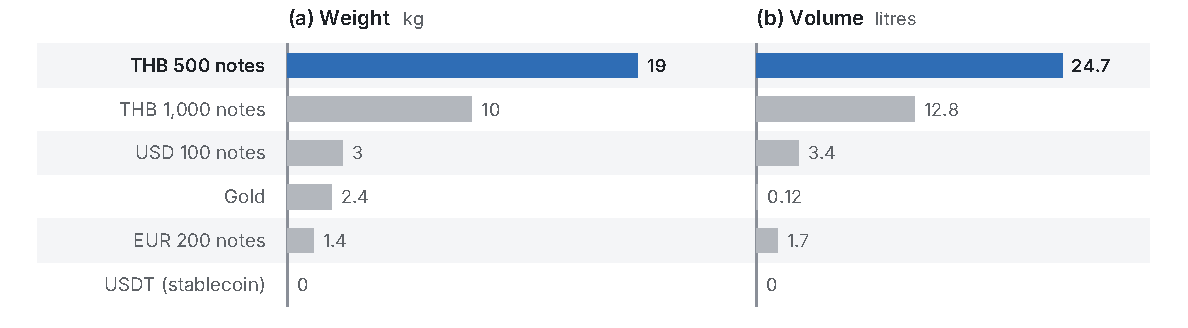
\includegraphics[width=\figw]{figs_en/bulk.pdf}
\caption{\textbf{Withdrawing the note doubles the bulk of large cash payments but leaves compact substitutes untouched.} (a)~Weight and (b)~volume of THB~10 million in each form; blue bars show the state after withdrawal. In 100-baht notes the same sum would weigh 90~kg and fill 119~litres. Notes weigh about one gram and are 0.11~mm thick; THB~33 per USD, USD~1.15 per EUR and USD~4,000 per troy ounce of gold. Source: \texttt{bulk\_table()} in the replication code.}\label{fig:bulk}
\end{figure}

Table~\ref{tab:channels} assesses how much Thailand's main illicit channels rely on the note. The assessment is
qualitative and is itself a hypothesis (H3 in Section~\ref{sec:framework}); much of the modern ``grey capital'' economy,
notably call-centre scams and online gambling, runs through mule accounts and crypto-assets rather than cash.

\begin{table}[!htbp]\centering\footnotesize
\caption{Reliance of illicit channels on the 1,000-baht note (author's assessment)}\label{tab:channels}
\begin{tabularx}{\textwidth}{@{}p{3.6cm}Yp{4.2cm}@{}}
\toprule
Channel & Reliance on 1,000-baht notes & Expected effect of withdrawal\\
\midrule
Call-centre and online scams & Low: funds move through mule accounts into crypto-assets & Negligible\\
Online gambling & Low: mule accounts and e-wallets & Negligible\\
Narcotics & Medium: cash at retail level; crypto and informal remittance at wholesale level & Higher short-run
transport costs\\
Bribery and corruption & Medium to high: large cash transfers, but final stores are assets and nominees & Harder delivery;
converted assets untouched\\
Vote buying & Low to medium: per-capita payments of hundreds to a few thousand baht & Small; substitution to 500s, transfers,
in-kind gifts\\
Tax evasion by cash businesses & High for cash-held portion & Partial; most can be structured or converted\\
Foreign grey capital and nominees & Low: corporate accounts and real estate & Negligible\\
\bottomrule
\end{tabularx}
\end{table}

Instruments that target illicit finance more directly already exist: the Currency Act B.E. 2501 (1958), under which the
authority to revoke legal-tender status must be examined; the Anti-Money Laundering Act B.E. 2542 (1999), which requires
reporting of cash transactions above THB 2 million; the Emergency Decree on Measures for the Prevention and Suppression of
Technology Crimes B.E. 2566 (2023), which targets mule accounts; and a 2019 amendment of the Revenue Code that requires
financial institutions to report high-frequency electronic receipts. Thailand has no general cap on cash payments, unlike
several EU member states and the forthcoming EU-wide limit \citep{amlr2024}. On the cost side, Thailand is an aged society
(roughly one in five citizens is 60 or older), about half of employment is informal, many farmers sell output for cash,
several million migrant workers have limited bank access, and baht circulates in border economies of Lao PDR, Cambodia and
Myanmar. Digital payments are pervasive (PromptPay operates since 2017) but concentrated among urban, working-age users.

\section{Conceptual framework: the demonetization trilemma}\label{sec:framework}

\subsection{Environment}
Let $K$ denote the value of the notes to be demonetized and $s\in(0,1)$ the share held as illicit wealth, so that the
illicit stock is $S=sK$. A design specifies a notice period $L\ge 0$, an exchange window $W>0$ and a legal-tender rule:
under a shock legal tender lapses at announcement ($L=0$); under an announced design it lapses at the deadline; under a
phase-out it persists for years and the notes remain redeemable.

\textit{Laundering.} Illicit holders can convert notes into alternative stores of value (gold, foreign currency,
stablecoins, real assets) through intermediaries with aggregate capacity $c$ per day at proportional cost $f_c$, for as
long as notes are accepted; structure deposits through money mules with capacity $m$ per day at cost $f_m$; deposit
directly; declare under an amnesty at tax rate $t$; or abandon the notes. Let $\ell=c+m$ denote laundering capacity per day
and $T$ the period during which laundering channels operate ($T=L+W$).

\textit{Enforcement.} Deposits arrive at rate $K/W$ during the window. The authorities can scrutinize value $A$ per day
with quality $\kappa\in(0,1]$, so the audit probability per unit deposited is $a(W)=\min\{1,AW/K\}$, and an illicit unit
passing through the banking system is detected with probability $p=\kappa\,q\,a(W)$, where $q\le 1$ captures how much
harder structured deposits are to flag.

\textit{Replacement.} When legal tender lapses, a share $R_0$ of the withdrawn value has already been replaced;
replacement then proceeds at rate $r$ per day.

\textit{Objectives.} The state cares about the \textit{bite} $B$, the share of $S$ extinguished or captured; the
\textit{disruption} $D$ imposed on honest holders; and the \textit{laundering share} $\Lambda$, the share of $S$ that
enters the financial system undetected.

\begin{assumption}[Anonymity]\label{ass:anon} The state cannot identify illicit holdings before they are presented for
exchange.\end{assumption}
\begin{assumption}[Finite capacities]\label{ass:cap} Audit capacity $A$, laundering capacity $\ell$ and the replacement
rate $r$ are finite.\end{assumption}
\begin{assumption}[Rational holders]\label{ass:rat} Each illicit holder chooses the channel that maximizes expected
retained value; detection destroys a share $\pi$ of the amount, with $\pi>1$ for criminal proceeds, which carry sanctions
beyond confiscation.\end{assumption}

\begin{lemma}[Liquidity gap]\label{lem:gap} If legal tender lapses when a share $R_0$ of the withdrawn currency has been
replaced and replacement proceeds linearly at rate $r$, the cumulative shortfall is
\begin{equation}
G=\int_0^\infty\left(1-R_0-rt\right)^{+}dt=\frac{(1-R_0)^2}{2r},
\end{equation}
and disruption is $D=\phi\,G$, where $\phi=s_{\mathrm{dem}}\sum_h w_h d_h(1-g_h)$ weights the shortfall by the
demonetized share of currency and by the cash dependence $d_h$ and digital readiness $g_h$ of transactions in group $h$
with weight $w_h$.\end{lemma}
\begin{proof} The integrand is positive on $[0,(1-R_0)/r)$ and the integral of a linear function over that interval is
$(1-R_0)^2/(2r)$.\end{proof}

\begin{proposition}[Notice erodes the bite]\label{prop:notice} Suppose laundering weakly dominates the alternatives for
every holder, $(1-f)(1-p_\ell\pi)\ge\max\{1-p\pi,\,1-t,\,0\}$, where $f$ and $p_\ell$ are the cost and detection
probability of the laundering channel. If laundering capacity covers the illicit stock, $\ell T\ge S$, then no illicit unit
is abandoned and the bite is bounded by the detection probability in laundering channels: $B\le p_\ell$.\end{proposition}
\begin{proof} Under the stated inequality every holder weakly prefers laundering; with $\ell T\ge S$ the capacity
constraint never binds, so all units are laundered. Extinguishment is zero, and the captured share equals $p_\ell$ times
the confiscated share $\min\{\pi,1\}\le 1$.\end{proof}

\begin{proposition}[Congestion]\label{prop:congestion} If $W<K/A$, the audit probability $a(W)=AW/K$ is strictly
increasing in $W$. Shortening the window to deny laundering time therefore lowers the probability that a deposited unit is
examined and raises the undetected share $1-\kappa qAW/K$ of illicit value passing through the banking system.\end{proposition}
\begin{proof} Immediate from $a(W)=AW/K<1$.\end{proof}

\begin{proposition}[Demonetization trilemma]\label{prop:trilemma} Fix thresholds $\bar b>p_\ell$, $\bar d>0$ and
$\bar\lambda\in(0,1)$, and suppose that a positive share of illicit value passes through the banking system. Under
Assumptions~\ref{ass:anon}--\ref{ass:rat}, a design attains $B\ge\bar b$, $D\le\bar d$ and $\Lambda\le\bar\lambda$ only if
\begin{equation}
\text{(i)}\;\ \ell(L+W)<S,\qquad \text{(ii)}\;\ \kappa q\,\frac{AW}{K}\ge 1-\bar\lambda,\qquad
\text{(iii)}\;\ \frac{(1-R_0)^2}{2r}\le\frac{\bar d}{\phi}.
\end{equation}
Conditions (i) and (ii) are jointly feasible only if $A>(1-\bar\lambda)\,\ell/(\kappa q s)$: audit capacity must exceed
laundering throughput scaled by the inverse illicit share. Under a shock, condition (iii) requires
$R_0\ge 1-\sqrt{2r\bar d/\phi}$: replacement currency must be printed and distributed before the announcement. When either
requirement fails, at most two of the three objectives can be met.\end{proposition}
\begin{proof}[Proof sketch] Condition (i) follows from Proposition~\ref{prop:notice}: if $\ell(L+W)\ge S$ the bite cannot
exceed $p_\ell<\bar b$. For illicit value passing through banks the undetected share is $1-\kappa q\,a(W)$, so
$\Lambda\le\bar\lambda$ requires $a(W)\ge(1-\bar\lambda)/(\kappa q)$, which with $a(W)=AW/K$ yields (ii). Combining (i),
with $L\ge0$, and (ii) gives $(1-\bar\lambda)K/(\kappa qA)\le W<sK/\ell$, which is non-empty only under the stated bound
on $A$. Condition (iii) follows from Lemma~\ref{lem:gap}.\end{proof}

\begin{remark} The trilemma concerns designs that rely on the exchange of notes to separate illicit from licit holdings.
India's 2016 design partly satisfied (i), but scrutiny of the deposit flood was necessarily ex post and partial, and
replacement currency was far from sufficient; the predicted combination---low bite, high disruption, substantial
legitimization---is what the episode delivered. A phase-out relaxes (ii) and (iii) at the price of (i); Figure~\ref{fig:trilemma} summarizes the three corners.\end{remark}

\begin{figure}[!htbp]\centering
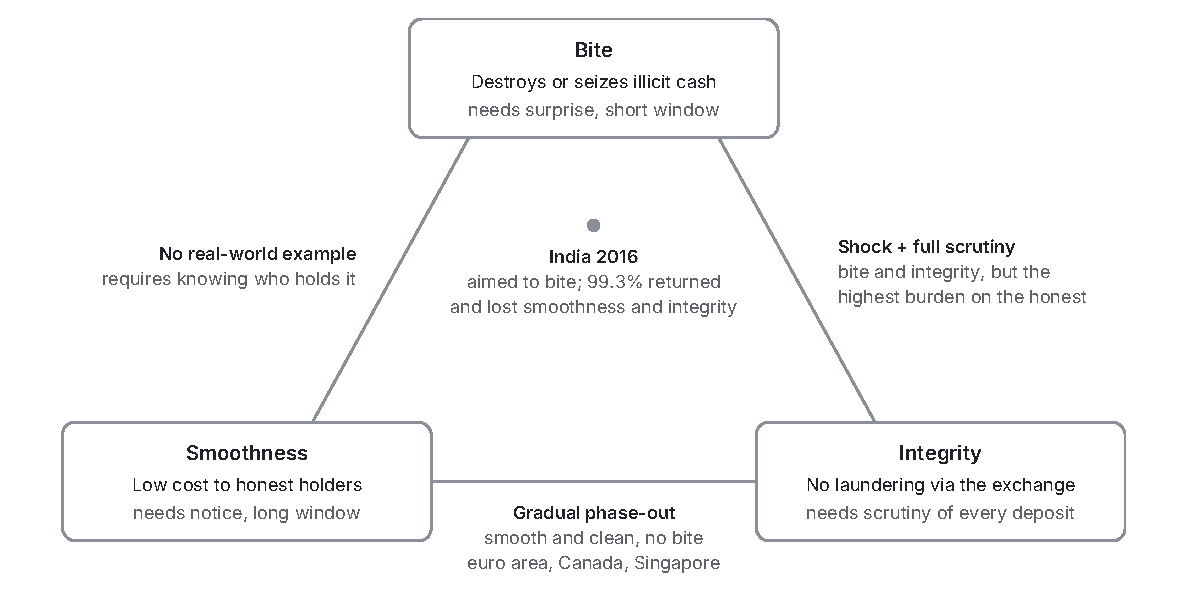
\includegraphics[width=\figw]{figs_en/trilemma.pdf}
\caption{\textbf{The demonetization trilemma: no design secures more than two of three goals.} Each side of the triangle is a design that secures the goals at its two ends and sacrifices the goal at the opposite vertex (Proposition~\ref{prop:trilemma}). India 2016 aimed at the bite but lost both smoothness and integrity.}\label{fig:trilemma}
\end{figure}

\subsection{Testable implications}
\begin{hypothesis}[Non-identification] Aggregate return rates do not identify $s$ when $\ell T$ is large relative to
$S$.\end{hypothesis}
\begin{hypothesis}[Capacity] The bite is decreasing in laundering capacity; scrutiny has first-order effects on the bite
only when $\ell T<S$.\end{hypothesis}
\begin{hypothesis}[Denomination premium] If the 1,000-baht note is a preferred illicit medium, its share in seized cash
exceeds its share in circulation.\end{hypothesis}
\begin{hypothesis}[Political money cycle] If vote buying relies on large notes, demand for 1,000-baht notes rises
disproportionately before elections.\end{hypothesis}

\noindent Hypotheses 1 and 2 are examined with the model in Section~\ref{sec:results}; Hypotheses 3 and 4 require new
data and motivate the designs in Section~\ref{sec:agenda}.

\section{DemonetSim-TH: model and calibration}\label{sec:model}

\subsection{Structure}
DemonetSim-TH is a partial-equilibrium Monte Carlo model with two modules. Uncertain parameters are drawn 600 times per
scenario; each draw simulates six groups of honest holders and 1,500 illicit agents. Parameter ranges are reported in
Appendix~\ref{app:model}.

\textit{Honest holders.} Group $h$ holds share $\sigma_h$ of the demonetized stock and has bank access $a_h$, digital
readiness $g_h$, cash dependence $d_h$ and transaction weight $w_h$ (Table~\ref{tab:holders}). The share converted before
the window closes is
\begin{equation}\label{eq:conv}
c_h=1-\exp\!\left(-\frac{a_h^{\mathrm{eff}}W}{\tau_0}\right),\qquad a_h^{\mathrm{eff}}=a_h\left[1-\tfrac12\kappa_b(1-a_h)\right],
\end{equation}
with $\tau_0=4$ days, so stricter documentation slows down holders with poor bank access. The disruption index applies
Lemma~\ref{lem:gap},
\begin{equation}\label{eq:index}
I=100\times\frac{s_{\mathrm{dem}}\sum_h w_h d_h(1-g_h)\,G}{\bar L_{\mathrm{IN16}}},
\end{equation}
where $R_0=\min\{1,\bar R_0+rW\}$ if legal tender persists to the deadline, $G=0$ under a phase-out, and
$\bar L_{\mathrm{IN16}}$ is the mean disruption of the India prior draws.

\textit{Illicit holders.} Holdings $x_i$, measured in units of the scrutiny threshold, are log-normal with
parameters $\ln 0.3$ and $1.8$, so that a small number of large holders own most illicit value. A holder is
``black'' (criminal proceeds) with probability $\beta$, in which case detection costs $\pi_i\sim U(1.5,3)$ times the amount,
or ``grey'' (undeclared legal income) with $\pi_i\sim U(0.6,0.9)$; the state recovers $\min\{\pi_i,1\}$. Perceived risk is
scaled by $\rho_i\sim\mathrm{LogNormal}(0,0.4)$. The values of the five channels are
\begin{equation}\label{eq:values}
\begin{aligned}
V_i^{\mathrm{dep}}&=1-p_i^{\mathrm{dep}}\pi_i, & p_i^{\mathrm{dep}}&=\kappa_b\left(1-e^{-x_i}\right)\rho_i,\\
V_i^{\mathrm{str}}&=(1-f_i^{s})\left(1-p_i^{\mathrm{str}}\pi_i\right), & p_i^{\mathrm{str}}&=\kappa_b\,q_s\,\rho_i,\\
V_i^{\mathrm{cnv}}&=(1-f_i^{c})\left(1-p_i^{\mathrm{cnv}}\pi_i\right), & p_i^{\mathrm{cnv}}&=\kappa_d\,q_c\,\rho_i,\\
V_i^{\mathrm{amn}}&=1-t\ \ (\text{grey holders only}), & V_i^{\mathrm{abn}}&=0,
\end{aligned}
\end{equation}
and holder $i$ chooses $k_i^*=\arg\max_{k\in\mathcal A_i}\left(V_i^k+\varepsilon_{ik}\right)$ with
$\varepsilon_{ik}\sim\mathrm{Gumbel}(0,0.02)$ \citep{mcfadden1974}. Structuring and conversion are capacity-constrained:
their capacities, expressed as shares of all demonetized cash over the operating period, are divided by $s$ to obtain
capacities relative to illicit holdings. Agents are processed in random order, and those who find their preferred channel
full fall back to their next-best option (Appendix Table~\ref{alg:alloc}). Detected deposits are captured or regularized after
penalty; undetected deposits and structured deposits net of fees are \textit{laundered}; conversions and fees are
\textit{displaced}; abandoned notes are \textit{extinguished}. The bite is extinguished plus captured value, and the return
rate is $1-s\times\text{extinguished}-\text{honest value not converted}$.

\subsection{Scenarios}
Table~\ref{tab:scenarios} defines four Thai scenarios and the India calibration scenario. S2 captures the main Nigerian
risk---insufficient replacement currency at the deadline---through a wide range for $\bar R_0$ and $r$; S4 adds a package of
cash-payment caps, enhanced due diligence on gold, crypto and property purchases and a crackdown on mule accounts, modeled as
higher detection and lower laundering capacity.

\begin{table}[!htbp]\centering\footnotesize
\caption{Scenarios}\label{tab:scenarios}
\begin{tabularx}{\textwidth}{@{}p{1.1cm}p{4cm}Y@{}}
\toprule
Code & Scenario & Key features\\
\midrule
S1 & Shock (India-style) & Legal tender lapses at once; 50-day window; amnesty at 50--60\% tax\\
S2 & Announced, 90-day deadline & Usable until the deadline; no amnesty; outcome depends on printing enough 500-baht notes\\
S3 & Phase-out, 5 years & Issuance stops; legal tender for five years; redeemable at the central bank indefinitely\\
S4 & Phase-out + AML package & S3 plus cash-payment cap, enhanced due diligence on dealers, mule-account crackdown\\
IN16 & India 2016 (calibration) & Indian parameters; draws retained by ABC if the simulated return rate is $99.3\pm0.3\%$\\
\bottomrule
\end{tabularx}
\end{table}

\subsection{Calibration and sensitivity analysis}
We treat India 2016 as the calibration target. We draw 4,000 parameter vectors from the IN16 priors, simulate the return
rate, and retain draws with $|\hat R-0.993|\le0.003$ \citep{beaumont2002}. Of the 4,000 draws, 1,214 (30.3 percent) are
accepted. To understand which inputs drive the outcomes, we compute partial rank correlation coefficients (PRCC) between
each of 13 sampled parameters and three outcomes across the 600 S1 draws \citep{marino2008}. PRCCs measure the monotone
association between an input and an outcome after removing the linear effects of all other inputs on the ranks; with 39
coefficients estimated from 600 draws, values below about 0.15 in absolute value are within sampling noise.

\section{Results}\label{sec:results}

\subsection{Bite versus disruption}
Table~\ref{tab:main} and Figure~\ref{fig:bite} report the central results. A Thai shock (S1) produces a disruption index of
17 against 97 for calibrated India---about one sixth---because the 1,000-baht note is a smaller share of currency and
digital readiness is far higher. Incidence is nonetheless highly regressive: about 91 percent of the disruption falls on
vulnerable households and informal businesses (81 percent in India). Honest holders fail to convert about 0.28 percent of
the stock, roughly THB 3.9 billion, three quarters of it held across the border. S2 is benign at the median but reaches an
index of about 10 in the worst decile of replacement outcomes, which is precisely the Nigerian failure mode.

\begin{table}[!htbp]\centering\footnotesize
\caption{Main simulation results}\label{tab:main}
\begin{threeparttable}
\begin{tabularx}{\textwidth}{@{}lYYYYY@{}}
\toprule
& Disruption index & Bite (\%) & Laundered (\%) & Displaced (\%) & Return rate (\%)\\
\midrule
IN16 (calibrated) & 96.8 [85.4, 113.2] & 8.5 [6.2, 12.0] & 60.2 & 27.8 & 99.50\\
S1 Shock & 17.2 [13.2, 23.9] & 7.7 [5.5, 15.4] & 60.9 & 25.2 & 99.63\\
S2 Announced, 90 days & 0.4 [0.0, 3.8] & 3.4 [2.7, 4.1] & 30.0 & 65.5 & 99.98\\
S3 Phase-out & 0.0 [0.0, 0.0] & 1.0 [0.9, 1.2] & 52.9 & 45.8 & 100.00\\
S4 Phase-out + AML & 0.0 [0.0, 0.0] & 6.1 [4.8, 7.5] & 67.4 & 24.7 & 100.00\\
\bottomrule
\end{tabularx}
\begin{tablenotes}\scriptsize
\item \textit{Notes:} Medians with interquartile ranges in brackets over 600 draws per scenario (IN16: ABC-accepted
draws). Laundered and displaced are means, in percent of the illicit stock. Bootstrap standard errors of the medians
(1,000 resamples) are 0.25 pp for the S1 and IN16 bites, 0.09 pp for S4, and 0.42 for the S1 disruption index.
\end{tablenotes}
\end{threeparttable}
\end{table}

\begin{figure}[!htbp]\centering
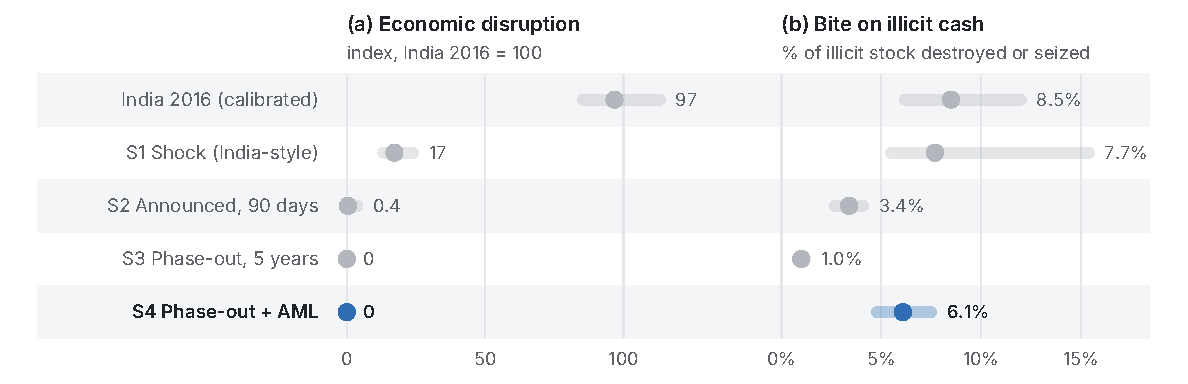
\includegraphics[width=\figw]{figs_en/bite.pdf}
\caption{\textbf{A phase-out with AML measures bites nearly as hard as a shock at no liquidity cost.} (a)~Economic disruption, indexed to the mean India 2016 prior draw (= 100). (b)~Share of illicit cash destroyed or seized. Dots are medians and bars interquartile ranges over 600 Monte Carlo draws per scenario; S4 is highlighted. Source: DemonetSim-TH, \texttt{scenario\_summary.csv}.}\label{fig:bite}
\end{figure}

The median bite of a shock is 7.7 percent; a phase-out combined with AML measures attains 6.1 percent at no liquidity
cost. The comparison should not be over-read: S4's bite stems from assumed improvements in detection that could be pursued
without withdrawing the note. What the phase-out adds is to force the stock through that tighter net within a known
horizon.

\subsection{Where illicit cash goes}
Figure~\ref{fig:fate} decomposes the fate of illicit cash. In every scenario most of it survives: between 30 and 67
percent enters the banking system undetected and between 25 and 65 percent is displaced into gold, foreign currency and
crypto-assets or absorbed as fees by laundering intermediaries. Advance notice (S2) maximizes displacement, because notes
remain spendable while holders buy alternative assets. Amnesty is almost never used (about 1 percent of illicit value): at
50--60 percent it is more expensive than laundering, which matches the weak take-up of India's 2016 scheme. The
distribution of the bite is right-skewed; in the best decile of draws a shock destroys or seizes more than 24 percent,
which happens only when the illicit stock is large and laundering capacity scarce.

\begin{figure}[!htbp]\centering
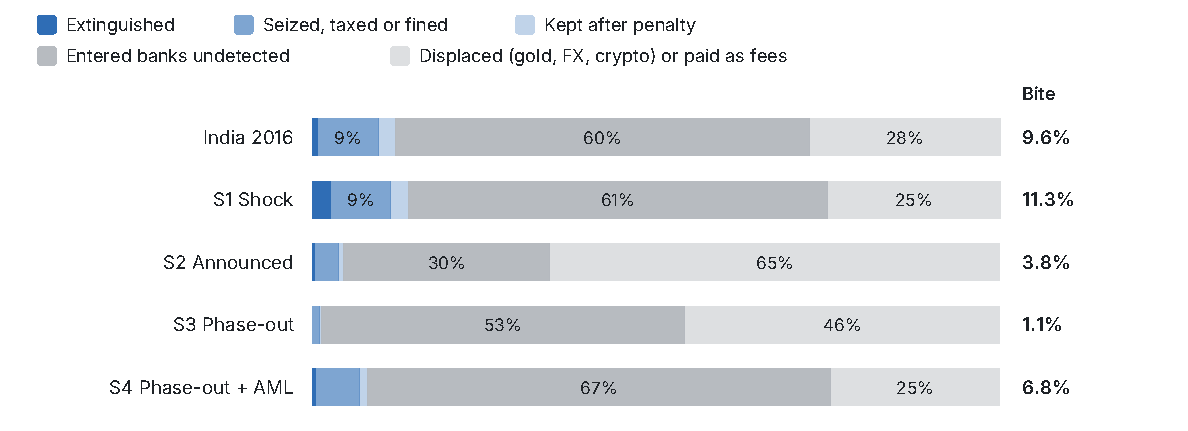
\includegraphics[width=\figw]{figs_en/fate.pdf}
\caption{\textbf{Most illicit cash survives: only 1--11\% is destroyed or seized in any scenario.} Value-weighted means across draws, hence above the medians in Figure~\ref{fig:bite}. Blue segments are gains to the state; grey segments are illicit value that survives. The bite is the sum of extinguished and seized value. Source: DemonetSim-TH, \texttt{mc\_results.csv}.}\label{fig:fate}
\end{figure}

\subsection{What India's return rate can and cannot tell us}\label{sec:ident}
Figure~\ref{fig:calib} plots the simulated return rate against the assumed illicit share for the India prior draws. The
acceptance region overlaps the simulated distribution at every illicit share between 3 and 29 percent. Table~\ref{tab:abc}
compares prior and posterior distributions: the posterior median of the illicit share (13.0 percent) barely differs from
the prior (15.7 percent), and the 10--90 percent interval shrinks only from 4.8--27.1 to 4.2--25.9 percent. The return rate
does trim the upper tail of the bite, from 23.8 to 15.9 percent at the 90th percentile. In short, the 99.3 percent
statistic rules out large-scale extinguishment, but it is nearly uninformative about the illicit stock (Hypothesis 1).

\begin{figure}[!htbp]\centering
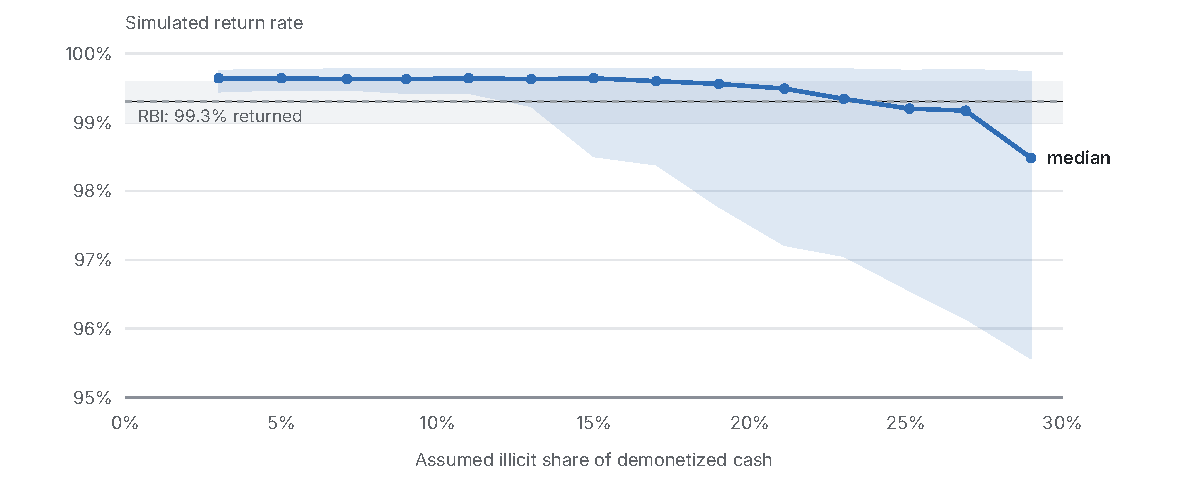
\includegraphics[width=\figw]{figs_en/calib.pdf}
\caption{\textbf{India's 99.3\% return rate fits any illicit share between 3\% and 29\%.} Simulated return rates from 4,000 draws of the India priors, grouped by the assumed illicit share; the line is the median, the blue band the 10th--90th percentile range and the grey band the ABC acceptance region ($99.3\pm0.3\%$). Sources: DemonetSim-TH, \texttt{india\_calibration\_curve.csv}; the target is from \citet{rbi2018}.}\label{fig:calib}
\end{figure}

\begin{table}[!htbp]\centering\footnotesize
\caption{Approximate Bayesian computation: prior versus posterior}\label{tab:abc}
\begin{tabular}{@{}lcc@{}}
\toprule
Quantity (\%) & Prior: median [p10, p90] & Posterior: median [p10, p90]\\
\midrule
Illicit share of demonetized cash, $s$ & 15.7 [4.8, 27.1] & 13.0 [4.2, 25.9]\\
Bite & 9.3 [5.0, 23.8] & 8.5 [4.7, 15.9]\\
Laundered undetected & 61.8 [46.9, 73.9] & 62.0 [46.1, 72.8]\\
Displaced & 22.0 [12.6, 39.6] & 25.0 [14.3, 44.2]\\
\bottomrule
\end{tabular}
\par\smallskip\scriptsize\textit{Notes:} 4,000 prior draws; 1,214 accepted with $|\hat R-0.993|\le0.003$.
\end{table}

\subsection{The binding constraint: laundering capacity}
Figure~\ref{fig:capacity} fixes the illicit share at 10 percent and varies laundering capacity. When the laundering network
can absorb only 1 percent of demonetized cash during the window, stricter scrutiny raises the bite from 18 to 41 percent.
Once capacity exceeds about 7.5 percent---roughly the illicit stock net of conversion capacity---the bite falls to 5--7
percent irrespective of scrutiny, as Proposition~\ref{prop:notice} predicts (Hypothesis 2). Disrupting mule networks, cash
purchases of gold and peer-to-peer crypto markets is therefore a precondition for, not a complement to, any design that aims
at the stock.

\begin{figure}[!htbp]\centering
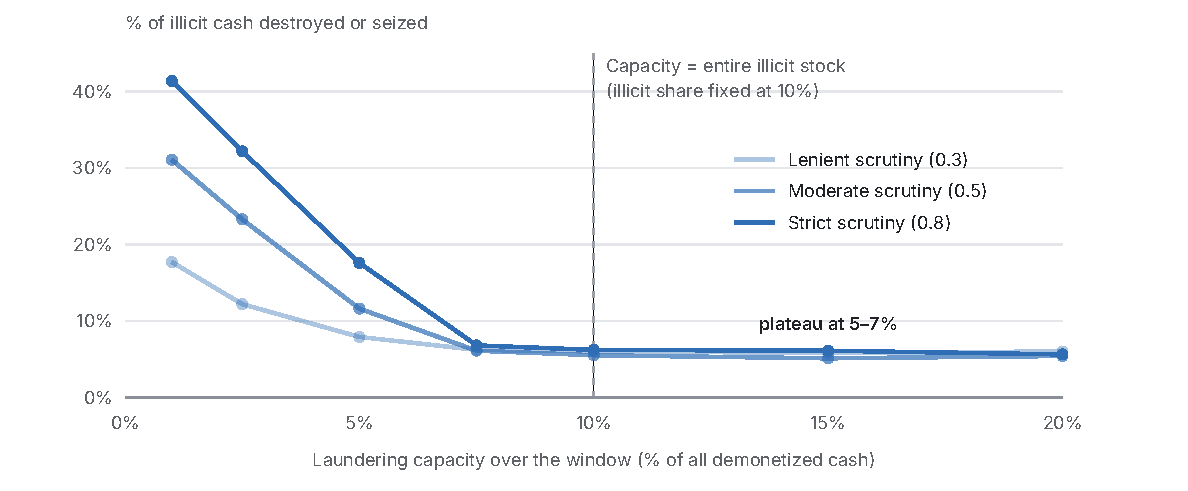
\includegraphics[width=\figw]{figs_en/capacity.pdf}
\caption{\textbf{Once laundering capacity exceeds the illicit stock, scrutiny barely matters.} Bite in scenario S1 as a function of laundering capacity over the exchange window, for three levels of bank scrutiny, with the illicit share fixed at 10\%; medians of 80 draws per point. The dashed line marks capacity equal to the illicit stock. Source: DemonetSim-TH, \texttt{sensitivity\_s1.csv}.}\label{fig:capacity}
\end{figure}

\subsection{Global sensitivity}
Figure~\ref{fig:prcc} reports PRCCs for the shock scenario. The bite is governed by the ratio of the illicit stock to
laundering capacity: the illicit share and structuring capacity have PRCCs of $+0.73$ and $-0.73$; the detectability of
structured deposits ($+0.33$) and the costs of structuring and conversion ($+0.22$, $+0.20$) follow, while bank scrutiny
intensity has a coefficient of only $+0.13$. The laundering share responds to capacity ($+0.71$), fees ($-0.54$) and
scrutiny ($-0.44$): scrutiny matters for integrity far more than for bite. Disruption depends almost exclusively on the
replacement rate ($-0.97$) and on currency ready on day zero ($-0.87$). The levers of bite and disruption are thus disjoint,
consistent with Lemma~\ref{lem:gap} and Proposition~\ref{prop:trilemma}.

\begin{figure}[!htbp]\centering
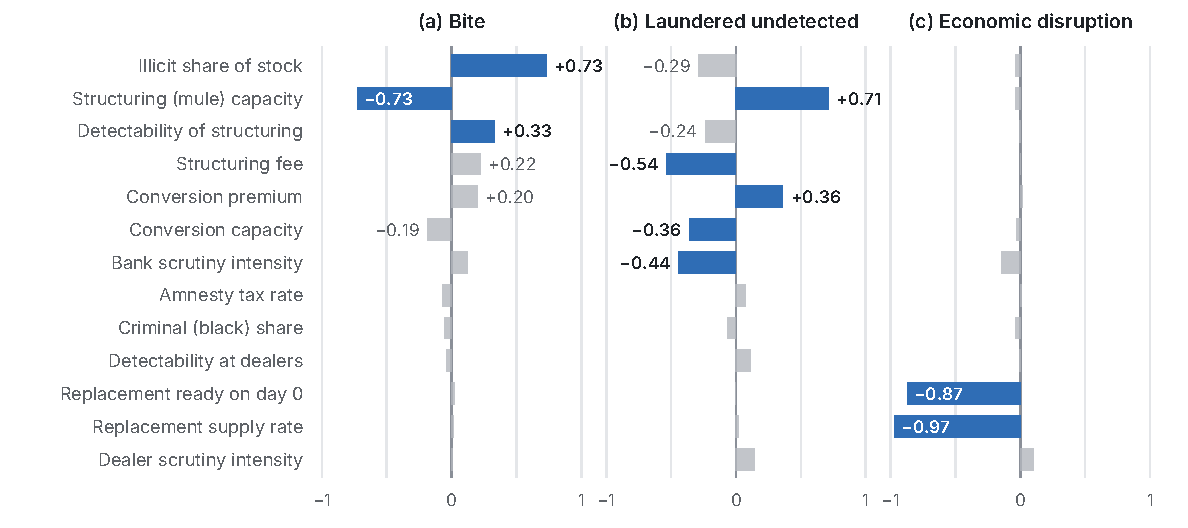
\includegraphics[width=\figw]{figs_en/prcc.pdf}
\caption{\textbf{Bite hinges on laundering capacity; disruption hinges on replacement logistics.} Partial rank correlation coefficients between each sampled parameter and (a)~the bite, (b)~the share laundered undetected and (c)~the disruption index, across 600 draws of scenario S1 \citep{marino2008}. Blue bars mark $|\mathrm{PRCC}|\ge0.3$; values below about 0.15 in absolute value are within sampling noise. Source: DemonetSim-TH, \texttt{prcc\_s1.json}.}\label{fig:prcc}
\end{figure}

\subsection{Operating costs}
Table~\ref{tab:costs} reports the operating costs of replacing the note. Together they amount to less than 0.1 percent of
GDP. The real costs of the policy are the disruption, its incidence and the risk to confidence in the baht, not printing.

\begin{table}[!htbp]\centering\footnotesize
\caption{Operating costs of replacing the 1,000-baht note}\label{tab:costs}
\begin{tabular}{@{}lcc@{}}
\toprule
Item & Median & 5th--95th percentile\\
\midrule
1,000-baht notes withdrawn (billion) & 1.37 & 1.19--1.58\\
500- and 100-baht notes printed (billion) & 2.27 & 1.76--2.83\\
Initial printing cost (THB billion) & 5.7 & 3.6--8.2\\
Additional annual printing cost (THB billion) & 0.8 & 0.2--1.7\\
Seigniorage shifted per year (THB billion) & 9.1 & 5.3--14.6\\
One-off ATM reconfiguration (THB billion) & 0.3 & 0.1--0.5\\
\bottomrule
\end{tabular}
\par\smallskip\scriptsize\textit{Notes:} 5,000 Monte Carlo draws over assumed ranges of currency in circulation, the
1,000-baht share, demand migration, unit printing costs, note lifetimes and interest rates.
\end{table}

\section{Assessment and policy design}\label{sec:policy}

\subsection{Costs and benefits}
Figure~\ref{fig:evidence} and Table~\ref{tab:proscons} position each claimed benefit and cost by impact and strength of
evidence. The largest costs---disruption of the informal economy and its regressive incidence---rest on strong evidence;
every benefit is either small or weakly evidenced. The strongest argument in favor of withdrawal is dynamic: without large
notes, bribery and hoarding become costlier every year, and societies may grow accustomed to traceable payments
\citep{rogoff2016,sands2016}. These flow effects lie outside the model and are a priority for research.

\begin{figure}[!htbp]\centering
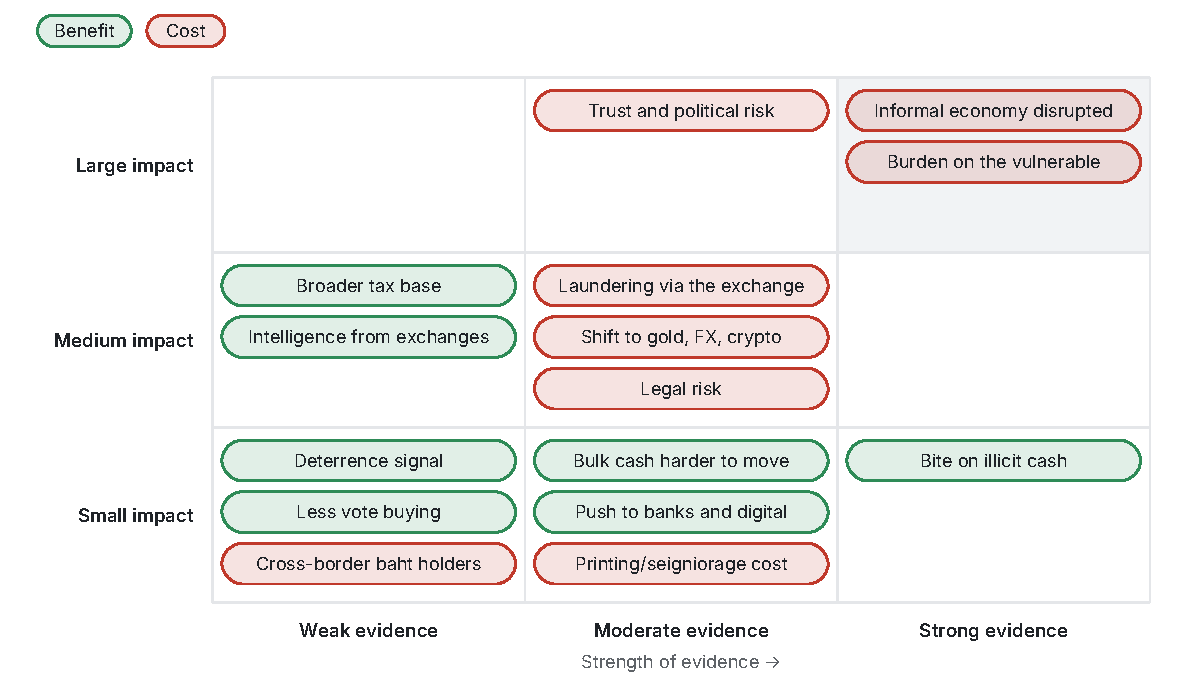
\includegraphics[width=\figw]{figs_en/evidence.pdf}
\caption{\textbf{The largest costs are well evidenced; every benefit is small or weakly evidenced.} Benefits (green) and costs (red) positioned by impact and strength of evidence; the shaded cell is the most worrying corner. Author's qualitative assessment, detailed in Table~\ref{tab:proscons}.}\label{fig:evidence}
\end{figure}

\begin{table}[!htbp]\centering\footnotesize
\caption{Benefits and costs of withdrawal (author's assessment)}\label{tab:proscons}
\begin{tabularx}{\textwidth}{@{}p{4.2cm}p{1.2cm}p{1.6cm}Y@{}}
\toprule
Item & Impact & Evidence & Basis\\
\midrule
\multicolumn{4}{@{}l}{\textit{Costs}}\\
Informal economy disrupted (shock) & Large & Strong & \citet{chodorowreich2020}\\
Burden on vulnerable groups & Large & Strong & India evidence; about 90\% of simulated disruption\\
Trust and political risk & Large & Moderate & Myanmar 1987, Soviet Union 1991, Venezuela 2016, Nigeria 2023\\
Laundering via the exchange & Medium & Moderate & 30--67\% of illicit cash enters banks undetected (model)\\
Displacement to gold, FX, crypto & Medium & Moderate & 25--65\% displaced (model)\\
Legal risk & Medium & Moderate & Indian (4--1) and Nigerian Supreme Court rulings\\
Printing and seigniorage & Small & Moderate & About THB 6 billion once and THB 10 billion a year\\
Cross-border baht holders & Small & Weak & No data\\
\addlinespace
\multicolumn{4}{@{}l}{\textit{Benefits}}\\
Broader tax base & Medium & Weak & Indian filings rose, confounded by the GST\\
Intelligence from exchanges & Medium & Weak & Depends on analytical capacity\\
Bite on illicit cash & Small & Strong & 99.3\% returned in India; 1--11\% in the model\\
Bulk cash harder to move & Small & Moderate & 10 to 19 kg per THB 10 million\\
Push to banks and digital payments & Small & Moderate & \citet{crouzet2023}; Thailand already highly digital\\
Deterrence signal & Small & Weak & No systematic evidence\\
Less vote buying & Small & Weak & Payments small; substitution to 500s and in-kind gifts\\
\bottomrule
\end{tabularx}
\end{table}

\subsection{Comparative evaluation}
Figure~\ref{fig:scorecard} scores five options against seven criteria. With equal weights the shock design scores lowest
(1.7 of 5) and the AML-based options highest (3.7--3.9). Doubling the weight on the bite makes the phase-out with AML (C+)
the top option; even with a fivefold weight on the bite, the shock design remains last. Because the scores are judgments,
the ranking should be read as a structured summary of the preceding evidence rather than as an independent result.

\begin{figure}[!htbp]\centering
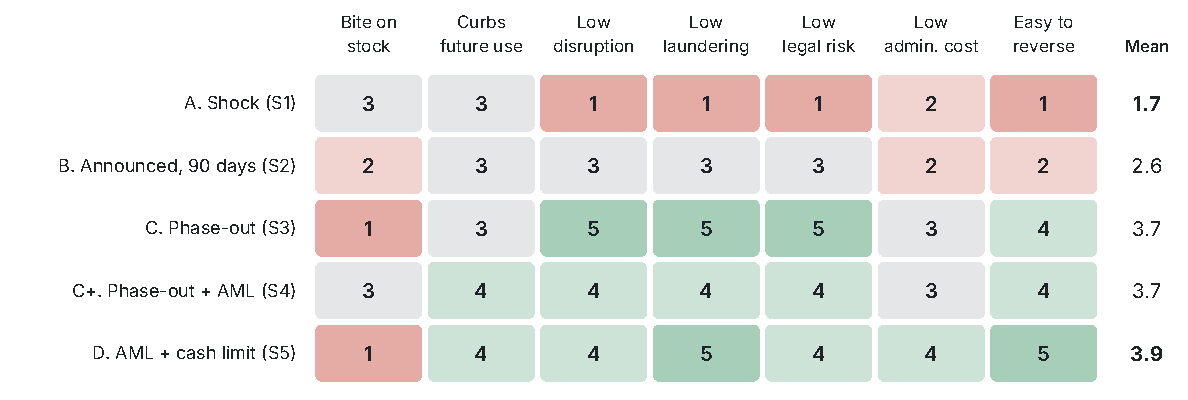
\includegraphics[width=\figw]{figs_en/scorecard.pdf}
\caption{\textbf{The shock design scores lowest; AML-based options score highest.} Author's scores from 1 (poor, red) to 5 (good, green) for five options against seven criteria; legal risk includes political risk, and the mean weights criteria equally. Options C and C+ phase out the 1,000-baht note; option D retains it.}\label{fig:scorecard}
\end{figure}

\subsection{A gated phase-out}
If the note is to be withdrawn, Figure~\ref{fig:roadmap} outlines a five-year phase-out with three decision gates at which
the process can be paused or reversed; reversal remains possible because the note stays legal tender until the final phase.
Five preconditions should be met before the first gate: (1) evidence that the note carries a premium in illicit use
(Section~\ref{sec:agenda}); (2) a demonstrable reduction in laundering capacity---mule accounts, cash purchases of gold,
peer-to-peer crypto markets and nominee structures; (3) adequate stocks of 500-baht notes and reconfigured ATMs; (4) a
statutory basis and exchange channels for the elderly, rural residents and holders in neighboring countries; and (5) an
independent evaluation plan with monthly open data by denomination. Four designs should be avoided: surprise
announcements; per-person exchange caps low enough to strand honest holders; simultaneous redesigns that create shortages;
and amnesties priced above market laundering fees, which attract almost no declarations.

\begin{figure}[!htbp]\centering
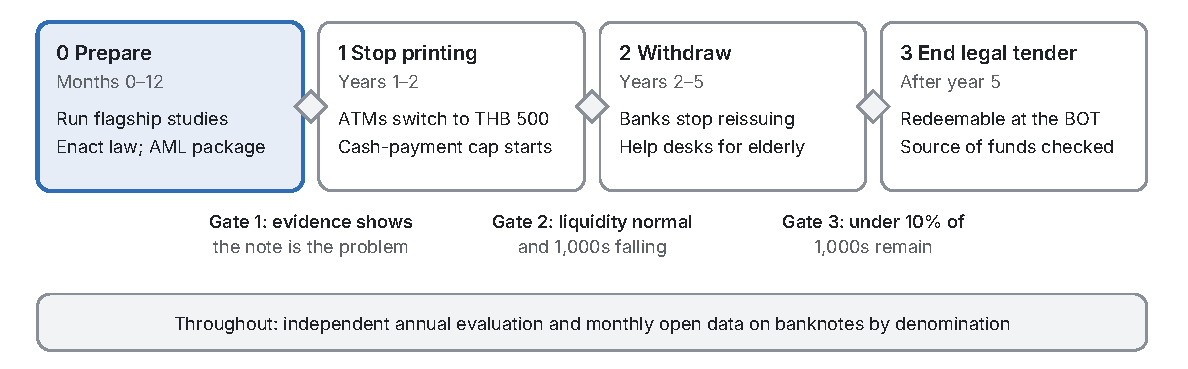
\includegraphics[width=\figw]{figs_en/roadmap.pdf}
\caption{\textbf{A gated five-year phase-out.} Phases are not drawn to scale. The blue frame marks what can start immediately; diamonds mark decision gates at which the process is paused or reversed if the criterion is not met. Author's proposal.}\label{fig:roadmap}
\end{figure}

\section{A research agenda}\label{sec:agenda}
Fifteen research topics follow from the analysis (Table~\ref{tab:agenda} and Figure~\ref{fig:agenda}). Three flagship
studies address the premise of the policy directly and are described in detail below.

\begin{table}[!htbp]\centering\scriptsize
\caption{Research agenda}\label{tab:agenda}
\begin{tabularx}{\textwidth}{@{}p{0.6cm}p{3.2cm}YY@{}}
\toprule
ID & Topic & Question & Design and data\\
\midrule
A1 & Who holds 1,000s & How much demand reflects transactions, hoarding or the informal economy? & Cash-demand models
(ARDL), note return frequencies; BOT data\\
A2 & Shadow economy & How has the shadow economy changed with digital payments? & MIMIC and currency-demand approaches
\citep{tanzi1983,medina2018}\\
A3$^\star$ & Pre-election cash & Does demand for 1,000s and 500s rise before elections? & Local projections, placebo dates;
monthly data by denomination\\
B1 & Cross-country & Which conditions make demonetization succeed or fail? & fsQCA \citep{ragin2008}; synthetic control
\citep{abadie2010}\\
B2 & Symbolic politics & Why choose low-yield, high-salience instruments? & Discourse and voting analysis\\
C1 & Distributional costs & Who bears the costs, and how much? & Microsimulation; household surveys\\
C2 & Public acceptance & Which designs do citizens accept? & Conjoint experiment \citep{hainmueller2014}\\
C3 & Cross-border baht & How much baht is held in Lao PDR, Cambodia, Myanmar? & Border-market surveys\\
D1$^\star$ & Seized-cash premium & Is the 1,000's share in seized cash above its circulation share? & Content analysis of
judgments and seizure reports\\
D2 & Vote-buying modes & Which notes, transfers or goods buy votes? & List experiment \citep{blair2012}\\
D3 & Displacement and mules & What is the laundering capacity of mule networks? & Network and on-chain analysis;
partnership data\\
E1 & Legal authority & Secondary legislation or an Act of Parliament? & Comparative law; proportionality\\
E2 & Cash caps & Do cash-payment caps shrink the shadow economy? & Natural experiments from Italian caps\\
F1$^\star$ & E-payment bunching & Do merchants stay below reporting thresholds and revert to cash? & Bunching estimation
\citep{saez2010,kleven2016}\\
F2 & Model extensions & Does the trilemma survive richer models? & ABM, heterogeneous-agent and game-theoretic models\\
\bottomrule
\end{tabularx}
\end{table}

\begin{figure}[!htbp]\centering
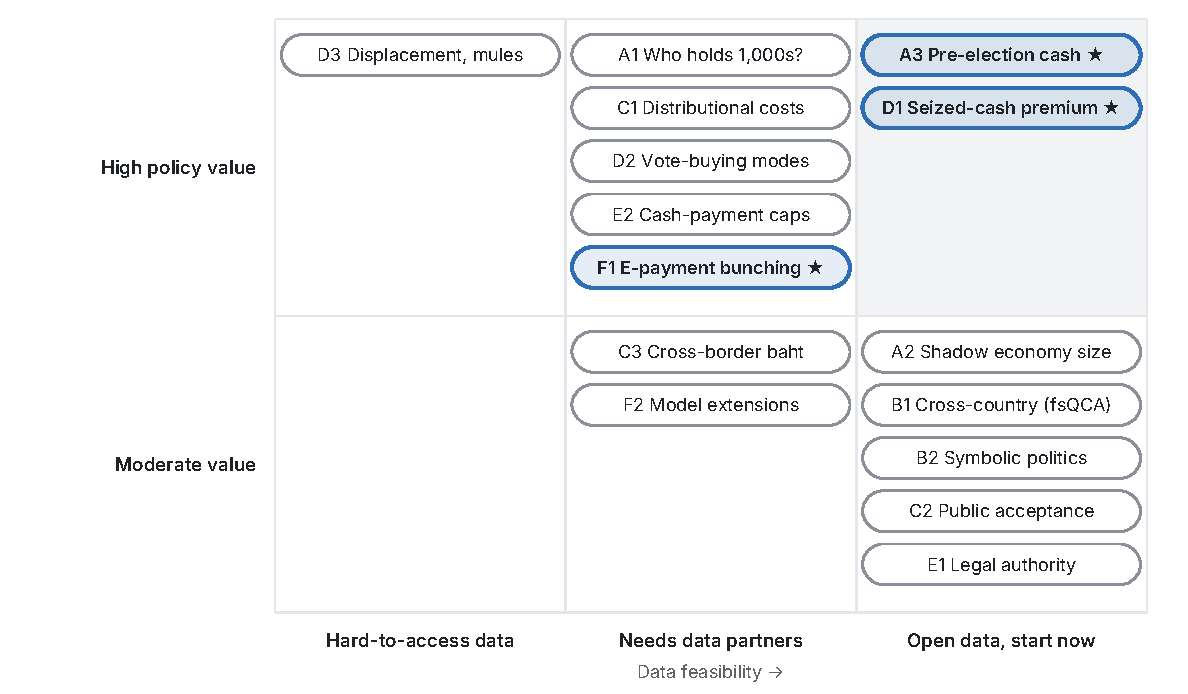
\includegraphics[width=\figw]{figs_en/agenda.pdf}
\caption{\textbf{Three flagship studies offer high policy value, and two can start with open data.} Fifteen research topics positioned by policy value and data feasibility; stars mark flagship studies and the shaded cell the topics to start with. Author's assessment; see Table~\ref{tab:agenda}.}\label{fig:agenda}
\end{figure}

\subsection{D1: an illicit denomination premium}
Let $y_c$ be the value share of 1,000-baht notes in the cash seized in case $c$, and $\pi^{\mathrm{circ}}_{t}$ the
share of the note in circulation at the seizure date $t(c)$. The estimand is the premium by crime type,
$\theta_k=E[y_c\mid k(c)=k]-\pi^{\mathrm{circ}}_{t(c)}$. We propose a fractional logit \citep{papke1996},
\begin{equation}
E[y_c\mid X_c]=\Lambda\!\left(\alpha+\textstyle\sum_k\beta_k\,\mathbf 1\{k(c)=k\}+\gamma_{t(c)}+\delta' Z_c\right),
\end{equation}
estimated on a sample of 300 to 1,000 judgments and seizure reports that record denominations, with region and enforcement-channel
controls $Z_c$. Hypothesis 3 predicts $\theta_k>0$ for bribery and wholesale narcotics. The main threat is selection into
detection; reporting estimates separately by detection channel and bounding the premium under alternative selection
assumptions mitigates it. A premium indistinguishable from zero would remove the empirical premise of the policy.

\subsection{A3: a political money cycle}
Let $C^d_t$ be notes in circulation of denomination $d\in\{100,500,1000\}$ in month $t$. Local projections
\citep{jorda2005},
\begin{equation}
\ln C^d_{t+h}-\ln C^d_{t-1}=\alpha^d_h+\beta^d_h E_t+\Gamma^{d\prime}_h X_t+\varepsilon^d_{t+h},\qquad h=0,\dots,H,
\end{equation}
trace the response to the pre-election period $E_t$, controlling for New Year, Chinese New Year and Songkran, the policy
rate and lags, and checked against placebo dates. With regional data, a difference-in-differences design interacts the
pre-election period with electoral competitiveness. If $\beta^{500}_h>0$ while $\beta^{1000}_h\approx0$, vote buying runs on
smaller notes and withdrawing the 1,000-baht note is mis-targeted (Hypothesis 4).

\subsection{F1: bunching at e-payment reporting thresholds}
Financial institutions report accounts that receive at least 3,000 electronic transfers a year, or at least 400 transfers
totaling THB 2 million (thresholds to be verified). If merchants avoid reporting by steering customers to cash, the
distribution of annual transfer counts will exhibit excess mass below the thresholds. Following \citet{saez2010},
\citet{kleven2013} and \citet{kleven2016}, the normalized excess mass is
\begin{equation}
\hat b=\frac{\sum_{j=z_L}^{z}\left(n_j-\hat n_j\right)}{\hat n(z)},
\end{equation}
where $n_j$ is the number of accounts in bin $j$, $\hat n_j$ the counterfactual from a polynomial fitted outside the
excluded window $[z_L,z_U]$ and $\hat n(z)$ the counterfactual density at the threshold $z$. Evidence of bunching would
indicate that tax-reporting rules push merchants back to cash, so currency and tax policy must be designed jointly.

\section{Limitations}\label{sec:limits}
Five limitations qualify the results. First, the Thai statistics are approximations that have not been verified against
primary sources. Second, the model is partial-equilibrium: it omits general-equilibrium feedbacks, dynamic responses of the
central bank and the long-run flow effects of retiring large notes, which are the strongest argument in favor of
withdrawal. Third, the illicit share is unknown; we therefore report results as distributions over wide priors, and the
India calibration shows that available aggregate data cannot narrow it. Fourth, detection is modeled in reduced form; in
particular, the compliance costs of the AML package in S4 for honest users are not quantified. Fifth, the scorecard and
the evidence map are qualitative judgments, and external validity of a calibration to India rests on the assumption that
laundering technologies are broadly similar.

\section{Conclusion}\label{sec:conclusion}
A shock withdrawal of the 1,000-baht note would likely do more harm than good: in the calibrated model it destroys or
seizes about 8 percent of illicit cash, concentrates about 90 percent of the disruption on vulnerable groups and turns the
exchange into a large-scale laundering channel. The note is not a large denomination by international standards, and
Thailand's grey capital increasingly moves through digital channels. The binding constraint on any design is the capacity
of laundering networks, which points to mule accounts, cash purchases of gold, peer-to-peer crypto markets and nominee
structures as the more promising targets, together with caps on cash payments. If withdrawal is nonetheless pursued, a
gated five-year phase-out preceded by the three flagship studies would test the premise before the costs are incurred.

\begin{thebibliography}{99}\small
\setlength{\itemsep}{1pt}
\bibitem[Abadie et~al.(2010)]{abadie2010} Abadie, A., Diamond, A., and Hainmueller, J. (2010). Synthetic control methods for comparative case studies. \textit{Journal of the American Statistical Association}, 105(490):493--505.
\bibitem[Bank of Thailand(various years)]{bot} Bank of Thailand (various years). Banknotes in circulation by denomination; Payment Systems Report. Bangkok.
\bibitem[Beaumont et~al.(2002)]{beaumont2002} Beaumont, M.~A., Zhang, W., and Balding, D.~J. (2002). Approximate Bayesian computation in population genetics. \textit{Genetics}, 162(4):2025--2035.
\bibitem[Bech et~al.(2018)]{bech2018} Bech, M., Faruqui, U., Ougaard, F., and Picillo, C. (2018). Payments are a-changin' but cash still rules. \textit{BIS Quarterly Review}, March.
\bibitem[Becker(1968)]{becker1968} Becker, G.~S. (1968). Crime and punishment: An economic approach. \textit{Journal of Political Economy}, 76(2):169--217.
\bibitem[Blair and Imai(2012)]{blair2012} Blair, G. and Imai, K. (2012). Statistical analysis of list experiments. \textit{Political Analysis}, 20(1):47--77.
\bibitem[Chodorow-Reich et~al.(2020)]{chodorowreich2020} Chodorow-Reich, G., Gopinath, G., Mishra, P., and Narayanan, A. (2020). Cash and the economy: Evidence from India's demonetization. \textit{Quarterly Journal of Economics}, 135(1):57--103.
\bibitem[Crouzet et~al.(2023)]{crouzet2023} Crouzet, N., Gupta, A., and Mezzanotti, F. (2023). Shocks and technology adoption: Evidence from electronic payment systems. \textit{Journal of Political Economy}, 131(11).
\bibitem[European Central Bank(2016)]{ecb2016} European Central Bank (2016). ECB ends production and issuance of EUR 500 banknote. Press release, 4 May.
\bibitem[European Union(2024)]{amlr2024} European Union (2024). Regulation (EU) 2024/1624 on the prevention of the use of the financial system for the purposes of money laundering or terrorist financing.
\bibitem[Europol(2015)]{europol2015} Europol (2015). \textit{Why Is Cash Still King? A Strategic Report on the Use of Cash by Criminal Groups as a Facilitator for Money Laundering}. The Hague.
\bibitem[FATF and APG(2017)]{fatf2017} FATF and APG (2017). \textit{Anti-Money Laundering and Counter-Terrorist Financing Measures---Thailand: Mutual Evaluation Report}.
\bibitem[Hainmueller et~al.(2014)]{hainmueller2014} Hainmueller, J., Hopkins, D.~J., and Yamamoto, T. (2014). Causal inference in conjoint analysis. \textit{Political Analysis}, 22(1):1--30.
\bibitem[Jobst and Stix(2017)]{jobst2017} Jobst, C. and Stix, H. (2017). Is cash back? Assessing the recent increase in cash demand. SUERF Policy Note 19.
\bibitem[Jord\`a(2005)]{jorda2005} Jord\`a, \`O. (2005). Estimation and inference of impulse responses by local projections. \textit{American Economic Review}, 95(1):161--182.
\bibitem[Kleven(2016)]{kleven2016} Kleven, H.~J. (2016). Bunching. \textit{Annual Review of Economics}, 8:435--464.
\bibitem[Kleven and Waseem(2013)]{kleven2013} Kleven, H.~J. and Waseem, M. (2013). Using notches to uncover optimization frictions and structural elasticities: Theory and evidence from Pakistan. \textit{Quarterly Journal of Economics}, 128(2):669--723.
\bibitem[Lahiri(2020)]{lahiri2020} Lahiri, A. (2020). The great Indian demonetization. \textit{Journal of Economic Perspectives}, 34(1):55--74.
\bibitem[Marino et~al.(2008)]{marino2008} Marino, S., Hogue, I.~B., Ray, C.~J., and Kirschner, D.~E. (2008). A methodology for performing global uncertainty and sensitivity analysis in systems biology. \textit{Journal of Theoretical Biology}, 254(1):178--196.
\bibitem[McFadden(1974)]{mcfadden1974} McFadden, D. (1974). Conditional logit analysis of qualitative choice behavior. In Zarembka, P. (ed.), \textit{Frontiers in Econometrics}, 105--142. Academic Press.
\bibitem[Medina and Schneider(2018)]{medina2018} Medina, L. and Schneider, F. (2018). Shadow economies around the world: What did we learn over the last 20 years? IMF Working Paper WP/18/17.
\bibitem[Olken and Pande(2012)]{olken2012} Olken, B.~A. and Pande, R. (2012). Corruption in developing countries. \textit{Annual Review of Economics}, 4:479--509.
\bibitem[Papke and Wooldridge(1996)]{papke1996} Papke, L.~E. and Wooldridge, J.~M. (1996). Econometric methods for fractional response variables with an application to 401(k) plan participation rates. \textit{Journal of Applied Econometrics}, 11(6):619--632.
\bibitem[Ragin(2008)]{ragin2008} Ragin, C.~C. (2008). \textit{Redesigning Social Inquiry: Fuzzy Sets and Beyond}. University of Chicago Press.
\bibitem[Reserve Bank of India(2018)]{rbi2018} Reserve Bank of India (2018). \textit{Annual Report 2017--18}. Mumbai.
\bibitem[Rogoff(1998)]{rogoff1998} Rogoff, K. (1998). Blessing or curse? Foreign and underground demand for euro notes. \textit{Economic Policy}, 13(26):261--303.
\bibitem[Rogoff(2016)]{rogoff2016} Rogoff, K.~S. (2016). \textit{The Curse of Cash}. Princeton University Press.
\bibitem[Saez(2010)]{saez2010} Saez, E. (2010). Do taxpayers bunch at kink points? \textit{American Economic Journal: Economic Policy}, 2(3):180--212.
\bibitem[Sands et~al.(2016)]{sands2016} Sands, P., Campbell, H., Keatinge, T., and Weisman, B. (2016). Making it harder for the bad guys: The case for eliminating high denomination notes. M-RCBG Associate Working Paper 52, Harvard Kennedy School.
\bibitem[Schneider and Enste(2000)]{schneider2000} Schneider, F. and Enste, D.~H. (2000). Shadow economies: Size, causes, and consequences. \textit{Journal of Economic Literature}, 38(1):77--114.
\bibitem[Stokes(2005)]{stokes2005} Stokes, S.~C. (2005). Perverse accountability: A formal model of machine politics with evidence from Argentina. \textit{American Political Science Review}, 99(3):315--325.
\bibitem[Supreme Court of India(2023)]{scindia2023} Supreme Court of India (2023). \textit{Vivek Narayan Sharma v.\ Union of India}, judgment of 2 January 2023.
\bibitem[Tanzi(1983)]{tanzi1983} Tanzi, V. (1983). The underground economy in the United States: Annual estimates, 1930--80. \textit{IMF Staff Papers}, 30(2):283--305.
\bibitem[Unger(2007)]{unger2007} Unger, B. (2007). \textit{The Scale and Impacts of Money Laundering}. Edward Elgar.
\bibitem[UNODC(2024)]{unodc2024} UNODC (2024). \textit{Casinos, Money Laundering, Underground Banking, and Transnational Organized Crime in East and Southeast Asia: A Hidden and Accelerating Threat}. Vienna.
\bibitem[Vicente(2014)]{vicente2014} Vicente, P.~C. (2014). Is vote buying effective? Evidence from a field experiment in West Africa. \textit{Economic Journal}, 124(574):F356--F387.
\end{thebibliography}

\appendix
\renewcommand{\thetable}{A\arabic{table}}\setcounter{table}{0}
\section{Model details}\label{app:model}

\begin{table}[!htbp]\centering\footnotesize
\caption{Holder groups: shares and behavioral parameters}\label{tab:holders}
\begin{tabular}{@{}lccccc@{\hspace{14pt}}ccccc@{}}
\toprule
& \multicolumn{5}{c}{Thailand} & \multicolumn{5}{c}{India 2016}\\
\cmidrule(lr){2-6}\cmidrule(l){7-11}
Group & $\sigma_h$ & $w_h$ & $a_h$ & $g_h$ & $d_h$ & $\sigma_h$ & $w_h$ & $a_h$ & $g_h$ & $d_h$\\
\midrule
Formal households & 0.32 & 0.30 & 0.95 & 0.85 & 0.35 & 0.20 & 0.20 & 0.80 & 0.30 & 0.60\\
Vulnerable households & 0.17 & 0.20 & 0.55 & 0.35 & 0.80 & 0.27 & 0.30 & 0.45 & 0.05 & 0.95\\
Formal firms & 0.08 & 0.25 & 1.00 & 0.90 & 0.25 & 0.08 & 0.20 & 1.00 & 0.50 & 0.40\\
Informal businesses & 0.20 & 0.25 & 0.60 & 0.50 & 0.85 & 0.30 & 0.30 & 0.55 & 0.05 & 0.95\\
Cross-border holders & 0.05 & 0.00 & 0.30 & 0.20 & 0.70 & 0.02 & 0.00 & 0.30 & 0.10 & 0.80\\
Banks and ATMs & 0.08 & 0.00 & 1.00 & 1.00 & 0.00 & 0.03 & 0.00 & 1.00 & 1.00 & 0.00\\
\bottomrule
\end{tabular}
\par\smallskip\scriptsize\textit{Notes:} $\sigma_h$: share of the demonetized stock (summing to 0.90 at an illicit share of
0.10 and rescaled otherwise); $w_h$: transaction weight; $a_h$: bank access; $g_h$: digital readiness; $d_h$: cash
dependence. Access, readiness and dependence receive $\pm15\%$ multiplicative noise in each draw.
\end{table}

\begin{table}[!htbp]\centering\footnotesize
\caption{Parameter ranges (uniform priors)}\label{tab:params}
\begin{tabular}{@{}lccccc@{}}
\toprule
Parameter & S1 & S2 & S3 & S4 & IN16\\
\midrule
Window or legal-tender period (days) & 50 & 90 & 1,825 & 1,825 & 50\\
Demonetized share of currency & 0.72 & 0.72 & 0.72 & 0.72 & 0.86\\
Bank scrutiny $\kappa_b$ & 0.35--0.65 & 0.30--0.60 & 0.20--0.40 & 0.50--0.80 & 0.25--0.55\\
Dealer scrutiny $\kappa_d$ & 0.20--0.40 & 0.20--0.40 & 0.10--0.30 & 0.50--0.80 & 0.10--0.30\\
Structuring fee $f^{s}$ & 10--30\% & 5--20\% & 0--3\% & 3--10\% & 15--35\%\\
Structuring capacity (\% of stock per day) & 0.05--0.30 & 0.05--0.25 & 0.008--0.022 & 0.003--0.008 & 0.05--0.40\\
Conversion premium $f^{c}$ & 15--40\% & 3--10\% & 1--4\% & 5--15\% & 15--40\%\\
Amnesty tax $t$ & 50--60\% & none & none & none & 50--60\%\\
Illicit share $s$ & 4--20\% & 4--20\% & 4--20\% & 4--20\% & 2--30\%\\
Replacement rate $r$ (\% per day) & 0.4--1.5 & 0.3--1.2 & -- & -- & 0.4--0.7\\
\bottomrule
\end{tabular}
\par\smallskip\scriptsize\textit{Notes:} Common to all scenarios: black share $\beta\sim U(0.25,0.60)$; detectability of
structuring $q_s\sim U(0.05,0.15)$ and of conversion $q_c\sim U(0.05,0.15)$ unless stated in the code; holdings
$\mathrm{LogNormal}(\ln0.3,1.8)$; $\tau_0=4$ days; Gumbel scale 0.02.
\end{table}

\begin{table}[!htbp]\centering\small
\caption{Capacity-constrained allocation}\label{alg:alloc}
\begin{tabularx}{\textwidth}{@{}rY@{}}
\toprule
1. & Draw holdings $x_i$, types, loss parameters $\pi_i$, risk multipliers $\rho_i$ and fees; compute $V_i^k$ from
(\ref{eq:values}) and add Gumbel noise.\\
2. & Set structuring and conversion capacities as shares of illicit holdings; draw a random processing order.\\
3. & For up to five rounds: each unassigned agent selects its best available channel. Unconstrained channels (deposit,
amnesty, abandonment) accept immediately; for each constrained channel, accept agents in processing order while cumulative
holdings do not exceed remaining capacity, and remove the channel from the choice set of rejected agents.\\
4. & Compute value-weighted shares of extinguished, captured, regularized, laundered and displaced value.\\
\bottomrule
\end{tabularx}
\end{table}

\section{Replication}\label{app:repl}
The model is implemented in \texttt{demonet\_sim\_th.py} (Python 3 with NumPy, pandas and Matplotlib). The command
\texttt{python demonet\_sim\_th.py --draws 600 --seed 7 --out out} reproduces all simulation results, writing ten CSV files
and six PNG figures; the PRCC coefficients are computed from \texttt{mc\_results.csv}. Before any policy use, the
denomination data, holder parameters, logistics ranges and scenario priors must be replaced with verified values; the
items most in need of verification are the stock of banknotes by denomination, the reporting thresholds under Thai AML
and tax law, and the episode-level figures in Table~\ref{tab:episodes}.

\end{document}
